\documentclass[tikz,margin=0.6mm]{standalone}

% pdftk jigsaw.pdf burst  output jigsaw%02d.pdf
% pdftocairo -singlefile -transp -r 250 -png jigsaw01.pdf jigsaw01

\usepackage{amsmath}
\usepackage{amssymb}
\usepackage{physics} % \usepackage[arrowdel]{physics}
\usepackage{txfonts} % times for math (for consistency)
\usepackage{times}
\usepackage{jigsaw}

\gdef\sigb{\vb*{\sigma}}
\gdef\taub{\vb*{\tau}}
\gdef\epsb{\dot{\vb*{\epsilon}}}
\gdef\eps#1{\dot{\epsilon}_{#1}}
\gdef\statevec{\vb{s}}
\gdef\bulkvisc{\vb*{\eta}}
\gdef\bulkvisc{E_{ij}}

%\gdef\mygray{black!9!white}
\definecolor{mydarkgray}{RGB}{200,200,200} 
\definecolor{mygray}{RGB}{240,240,240} 

\definecolor{colorFL}{RGB}{198,219,239} % flow law 
\definecolor{colorMB}{RGB}{218,218,235} % momentum balance
\definecolor{colorFM}{RGB}{199,233,192} % fabric model
\definecolor{colorVA}{RGB}{253,208,162} % viscous anisotropy

\gdef\asp{0.75}
\gdef\asp{0.85}
\gdef\scale{2.0}

\gdef\mylarge#1{ #1 }
\gdef\mysmall#1{ {\fontsize{6.0}{6.0}\selectfont #1} }

\tikzset{every picture/.style={line cap=rect,line width=0.6pt}}

\newcommand{\blockFL}[1]{
	\begin{scope}[xshift=0cm,yshift=1cm]
	    \color{black}
	    \piece[#1]{1}{-1}{0}{0}
	    \color{black}    
	    \node at (0.5,0.55) {\mylarge{$\taub(\epsb,\bulkvisc, \vb{m}_i, \cdots)$}};
	    \node[anchor=west] at ({(0)},{(0.9)}) {\mysmall{Bulk rheology}};
	\end{scope}   
}

\newcommand{\blockMB}[1]{
\begin{scope}[xshift=1cm,yshift=1cm]
    \color{black}
    \piece[#1]{-1}{0}{0}{1}
    \color{black}    
    \node at (0.630,0.53) {\mylarge{$-\div\sigb=\rho\vb{g}$}};
    \node at (0.630,0.37) {\mylarge{$\sigb=\taub-p\vb{I}$}};
    \node[anchor=east] at ({(1)},{(0.9)}) {\mysmall{Momentum balance}};
\end{scope}   
}

\newcommand{\blockFM}[1]{
\begin{scope}[xshift=1cm,yshift=0cm]
    \color{black}
    \piece[#1]{0}{0}{1}{-1}
    \color{black}
	\node at ({0.5},0.45) {\mylarge{$\dfrac{\mathrm{D} \statevec}{\mathrm{D} t} = \vb{M}\statevec$}};
    \node[anchor=east] at ({1},0.1) {\mysmall{Fabric evolution}};
\end{scope}    
}

\newcommand{\blockVA}[1]{
\begin{scope}[xshift=0cm,yshift=0cm]
    \color{black}
    \piece[#1]{0}{1}{-1}{0}
    \color{black}
	\node[align=left] at ({0.38},0.47) {\mylarge{$\bulkvisc(\statevec)$, $\vb{m}_i(\statevec)$}};
	\node[anchor=west,align=left] at ({0},0.10) {\mysmall{Viscous anisotropy}};
\end{scope}   
}


\begin{document}

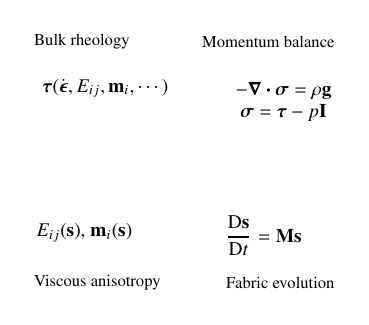
\begin{tikzpicture}[xscale=\scale,yscale={\scale*\asp}]
\scriptsize
\blockFL{colorFL}
\blockMB{colorMB}
\blockVA{colorVA}
\blockFM{colorFM}
\end{tikzpicture}

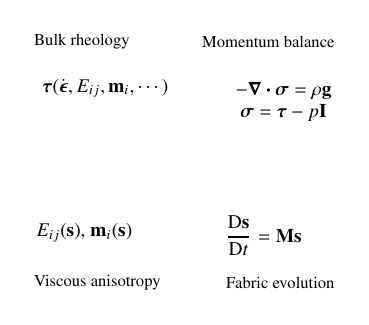
\begin{tikzpicture}[xscale=\scale,yscale={\scale*\asp}]
\scriptsize
\blockFL{mygray}
\blockMB{mygray}
\blockVA{mygray}
\blockFM{colorFM}
\end{tikzpicture}

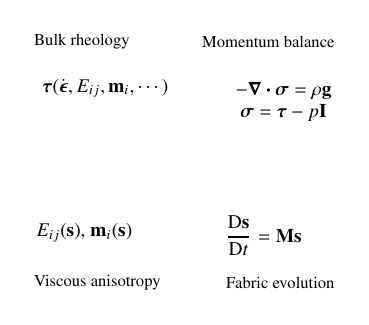
\begin{tikzpicture}[xscale=\scale,yscale={\scale*\asp}]
\scriptsize
\blockFL{mygray}
\blockMB{mygray}
\blockVA{colorVA}
\blockFM{mygray}
\end{tikzpicture}

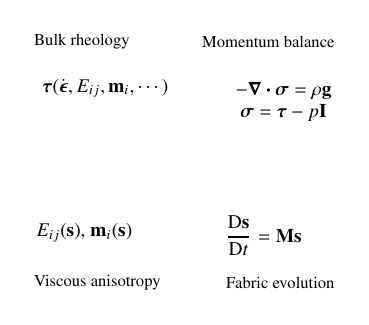
\begin{tikzpicture}[xscale=\scale,yscale={\scale*\asp}]
\scriptsize
\blockFL{colorFL}
\blockMB{mygray}
\blockVA{mygray}
\blockFM{mygray}
\end{tikzpicture}

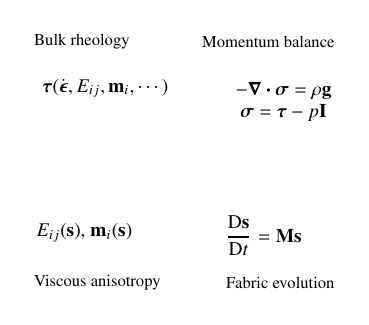
\begin{tikzpicture}[xscale=\scale,yscale={\scale*\asp}]
\scriptsize
\blockFL{mygray}
\blockMB{colorMB}
\blockVA{mygray}
\blockFM{mygray}
\end{tikzpicture}

\end{document}
